\item \textbf{{[}HCI/PRELIM/9597/2017/P1/Q4{]} }

The task is to store a dataset of students\textquoteright{} names
and test scores (max size of 20 students) as a binary tree structure.
The text file \texttt{SCORES.txt} stores the students\textquoteright{}
names and test scores in the following format: 
\noindent \begin{center}
\texttt{<Student Name>|<Score> }
\par\end{center}

All test scores are integer values in the range 0 to 100 inclusive. 

The program will use a user-defined type \texttt{Node} for each node
defined as follows: 
\noindent \begin{center}
\begin{tabular}{|c|c|c|}
\hline 
\textbf{Identifier} & \textbf{Data Type} & \textbf{Description}\tabularnewline
\hline 
\texttt{LeftP} & \texttt{INTEGER} & The left pointer for the node\tabularnewline
\hline 
\texttt{Name} & \texttt{STRING} & The name of the student\tabularnewline
\hline 
\texttt{Score} & \texttt{INTEGER} & The score of the student\tabularnewline
\hline 
\texttt{RightP} & \texttt{INTEGER} & The right pointer for the node\tabularnewline
\hline 
\end{tabular}
\par\end{center}

A linked list is maintained of all the unused nodes which do not form
part of the tree. The first available node which is used for a new
student is indicated by \texttt{NextFreePosition}. Nodes in the unused
list are linked using their left pointers.

The binary tree and linked list are implemented using variables as
follows:
\noindent \begin{center}
\begin{tabular}{|c|c|c|}
\hline 
\textbf{Identifier} & \textbf{Data Type} & \textbf{Description}\tabularnewline
\hline 
ThisTree & ARRAY{[}20{]}: Node & The tree data\tabularnewline
\hline 
Root & INTEGER & Index for the root position of the array\tabularnewline
\hline 
NextFreePosition & INTEGER & Index for the next unused node\tabularnewline
\hline 
\end{tabular}
\par\end{center}

\begin{center}
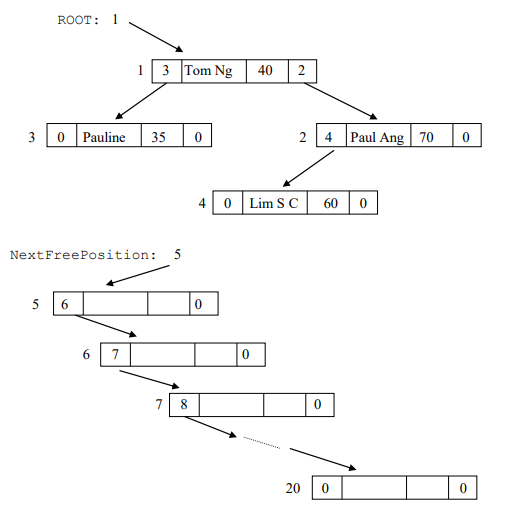
\includegraphics[width=0.5\paperwidth]{C:/Users/Admin/Desktop/Github/question_bank/LyX/static/img/9597-HCI-2017-P1-Q4-1}
\par\end{center}

The diagram shows the binary tree with the students\textquoteright{}
scores 40, 70, 35 and 60 (added in that order) and linked list of
unused nodes after the four students\textquoteright{} scores have
been added. 

\subsection*{Task 4.1 }

Write the program code to declare all the required variables and create
the initial linked list which contains all 20 nodes. Add statement(s)
to initialize the empty tree. 

\subsection*{Evidence 19 }

Your program code for Task 4.1. \hfill{}{[}8{]}

\subsection*{Task 4.2}

Write a non-recursive procedure \texttt{AddNodeToTree} to add a new
node with student\textquoteright s name and score into the binary
tree structure. 

\subsection*{Evidence 20}

Your program code for Task 4.2.\hfill{} {[}8{]}

\subsection*{Task 4.3 }

Write a procedure \texttt{OutputData} which displays the value of
\texttt{Root}, the value of \texttt{NextFreePosition} and the contents
of \texttt{ThisTree} in index order.

\subsection*{Evidence 21 }

Your program code for Task 4.3.\hfill{} {[}5{]}

\subsection*{Task 4.4 }

Write a main program to: 
\begin{itemize}
\item construct a binary search tree using the data provided in the text
file SCORES.txt by calling procedure \texttt{AddNodeToTree}. 
\item Your program will then call procedure \texttt{OutputData}. 
\end{itemize}

\subsection*{Evidence 22 }

Your program code for Task 4.4.\hfill{} {[}4{]}

\subsection*{Evidence 23 }

Screenshot showing the output from running the program in Task 4.4.\hfill{}
{[}4{]}

\subsection*{Task 4.5}

Write a recursive procedure \texttt{RankList} to output students\textquoteright{}
names and scores in descending scores order. Include a call to the
procedure from your main program. Evidence 24 Your program code for
Task 4.5.\hfill{} {[}4{]}

\subsection*{Evidence 25 }

Provide a screenshot showing students\textquoteright{} names and scores
in descending scores order. \hfill{}{[}2{]}